\section{Hub}
\subsection{Hub의 개념}
    Hub(허브)는 여러 대의 컴퓨터, 네트워크 장비를 연결하는 장치이다. 한대의 허브를 중심으로 여러대의 컴퓨터, 네트워크 장비가 성형 구조로 연결되며, 같은 허브에 연결된 컴퓨터와 네트워크 장비는 모두 상호 간에 통신할 수 있게 된다. \\
    허브로 연결된 네트워크에서는 한 컴퓨터에서 주고받는 데이터가 같은 허브에 연결된 다른 모든 컴퓨터에 전달되는데, 이를 Flooding이라고 한다. 허브는 본래 OSI 7계층의 1계층 장비로, 2계층의 MAC 주소로 송수신지를 구분할 수 없기 때문에 Flooding 방식을 이용한다. 통신은 데이터 전송시 송신 측은 데이터를 보내고 수신 측은 오직 송신 측에서 보낸 데이터만 받는 반이중 방식(Half Duplex)을 사용한다. \\
    \vspace{-4mm}
    \begin{figure}[!h]\centering
		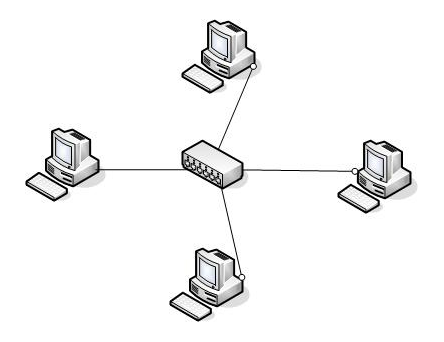
\includegraphics[width=.65\textwidth]{image/week05/3-1.png}
		\caption{\small Hub}
		\vspace{-10pt}
    \end{figure}
    
\subsection{Hub의 동작}
    이더넷 허브의 전송방식은 CSMA/CD(Carrier Sense Multiple Access, Collision Detection)로, 이는 반송파를 감지하며 네트워크의 다중 접속을 지원하는 기술이다. CSMA/CD는 전송 전에  다른 노드가 전송 중인지 확인하는 작업을 거쳐 노드끼리의 충돌 가능성을 줄여주며 패킷의 충돌을 방지한다. 다음과 같은 방식으로 순차적으로 진행한다.
    \begin{enumerate}
        \item 컴퓨터가 네트워크를 사용하기 전에 현재 네트워크에서 흐르고 있는 데이터패킷이 있는지 확인한다.  
        \item 네트워크상에 다른 데이터 패킷이 전송되고 있다면 데이터 전송이 끝나는 시점까지 기다리고 그렇지 않을 때에는 전송을 바로 진행한다.
        \item 여러 대의 PC가 동시에 데이터 패킷을 전송하여 데이터의 충돌이 발생하면 최소단위의 데이터 패킷을 다시 보내 다른 컴퓨터가 이를 알아차려 충돌을 방지 할 수 있게 한다.
        \item 데이터가 처리될 때까지 임의의 시간 동안 기다리고 다시 반송파를 보내 네트워크에 사용자가 없으면 전송을 재개한다.
        \item 원하는 전송을 클리어하면 상위계층에 이를 알리고 종료한다. 만약 이 과정을 여러 번 시도함에도 전송에 실패하면 이 역시도 상위 계층에 정보를 전송하고 종료한다.
    \end{enumerate}
\newpage